\begin{figure}
  \caption{\label{fig:pr_intern}Counts of linked individuals by their estimated internment `probability'}
  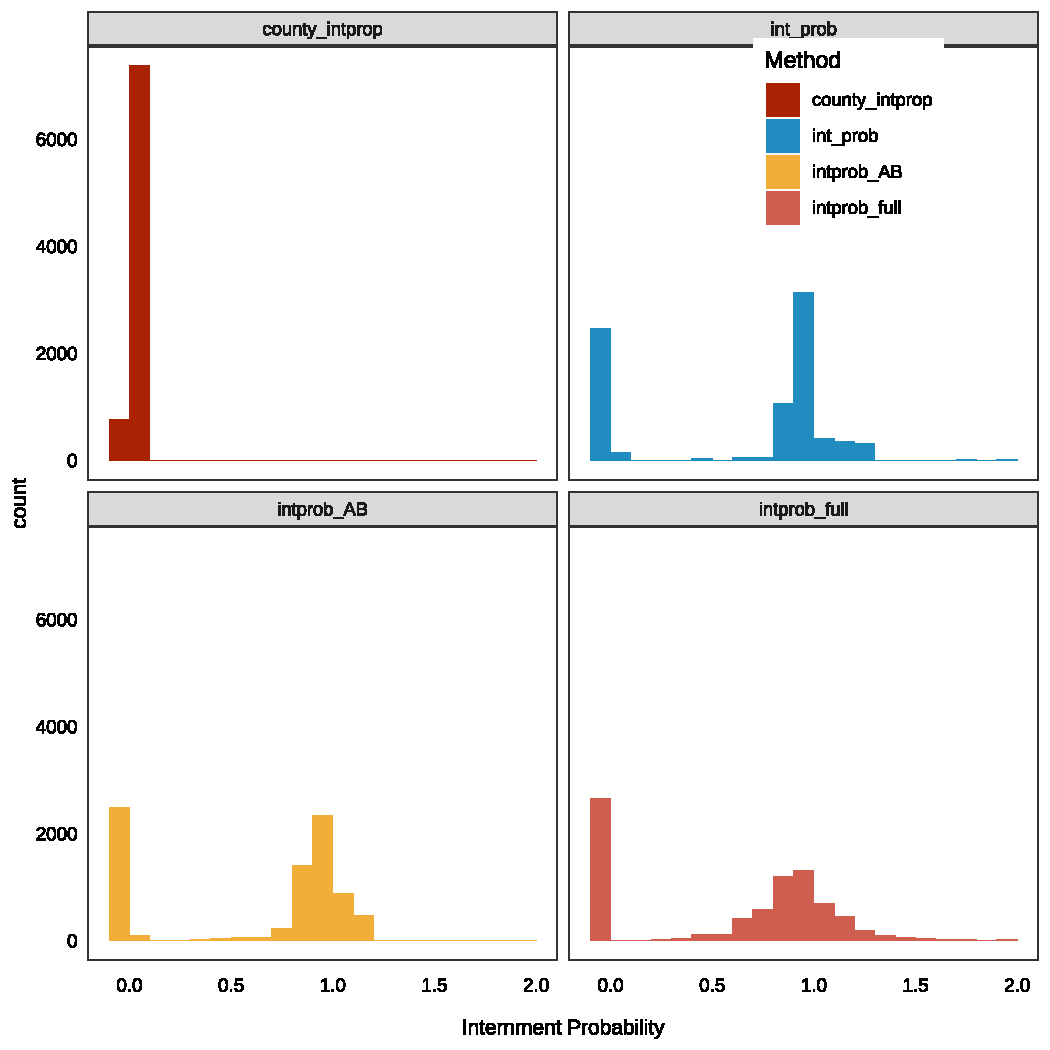
\includegraphics[width=.8\textwidth]{../figures/pr_intern_plot.pdf} \\
  \footnotesize
  This figure includes all Japanese and Chinese individuals who are linked across the 1940 and 1950 censuses
  in version 1.2 of the IPUMS MLP project.
  An individual's probability of being an internee is estimated as the ratio of interned people to the 
  number of people in the 1940 full-count census who have the same county and demographics.
  My cutoff for categorizing a person in the linked records as a likely internee is shown by the vertical line at 0.5.
\end{figure}
